
In this section, we know proceed to describe a real-world implementation of the
CAIS architecture described above. This implementation is open-sourced under the
name of BishopCAIS is available at \url{https://github.com/bishopcais}. A diagram
of the implemented modules is shown in Figure~\ref{fig:cais_implementation}, which includes
communication methods we use between each module. The modules are described below, giving detail on what
triggers these modules and their output. Three components, Reagent, 
spatial-context-bridge (which is described as part of Reagent), and MUIFOLD, are
described in the following two chapters to demonstrate their novelty in their
operation and functionality.


\begin{figure}
    \centering
    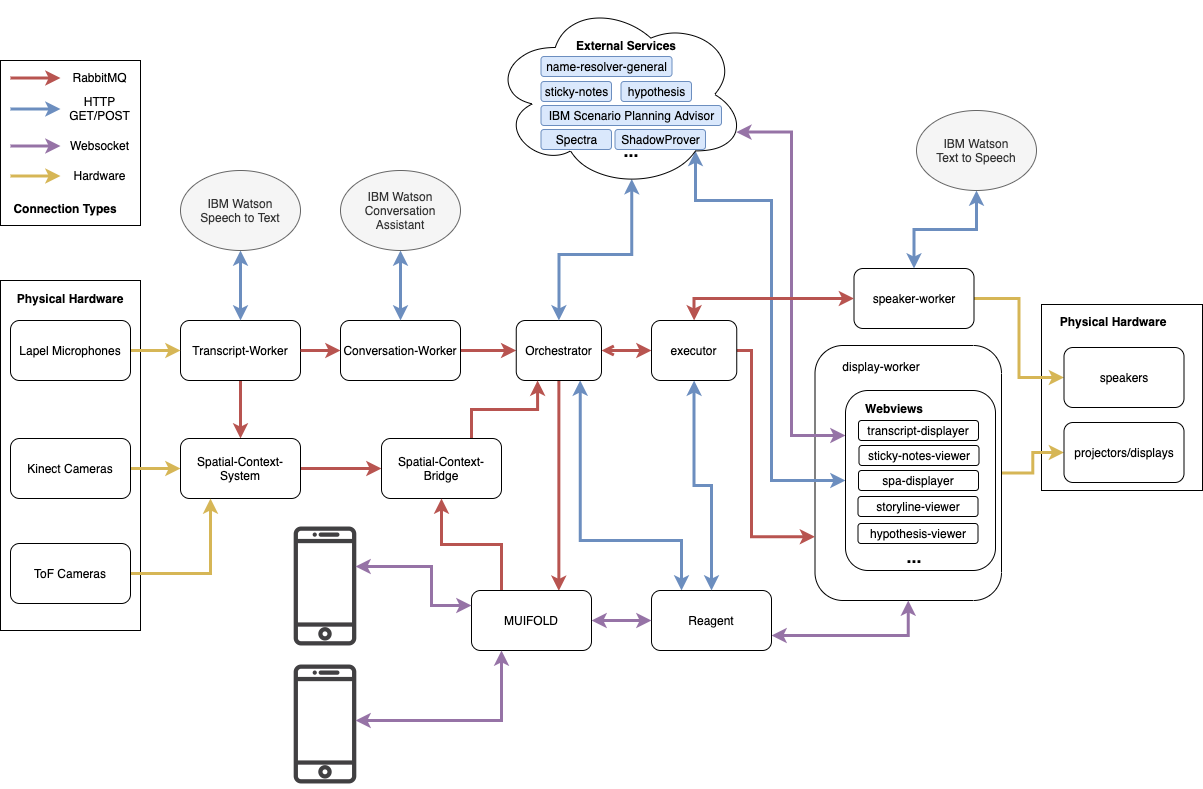
\includegraphics[width=1\columnwidth]{chapters/02_technology/figures/cais_implementation_full.png}
    \caption{Diagram of BishopCAIS Modules.}
    \label{fig:cais_implementation}
\end{figure}
